\chapter{Protocolli per lo scambio di chiavi}
Lo scambio (e la creazione) di chiavi crittografiche è un metodo che consente di scambiare le chiavi tra utenti, consentendo l'uso di un algoritmo crittografico. Se il mittente e il destinatario desiderano scambiarsi messaggi criptati, ciascuno deve possedere gli strumenti adatti per criptare e decriptare i messaggi inviati e ricevuti. La tipologia di chiavi di cui hanno bisogno dipende dalla tecnica di crittografia che hanno intenzione di utilizzare. Per esempio, se l'algoritmo di cifratura è a chiave simmetrica, entrambi avranno bisogno di una copia della stessa chiave. Se si tratta invece di un algoritmo a chiave asimmetrica, ognuno dei due avrà bisogno della chiave pubblica dell'altro.\\
Un protocollo per condividere una chiave segreta senza doverla scambiare, evitando quindi il pericolo di intercettazione, è noto come scambio di chiavi di \textbf{Diffie-Hellman} (1976).

\section{Scambio di chiavi Diffie-Hellman}
L'algoritmo Diffie-Hellman \cite{dh} poggia le proprie fondamenta sulla difficoltà di calcolare un \textbf{logaritmo discreto}, infatti, calcolare il valore $x = g^i$ $mod$ $n$ è facile, ma nessuno è acora stato in grado di individuare un metodo semplice per ricavare $i$ a partire da $g$, $x$ e $n$. Il protocollo è riassunto nei seguenti passaggi:
\begin{itemize}
    \item A sceglie due numeri primi molto grandi $n$ e $g$ con $(n-1)/2$ ancora primo, che possono essere resi noti senza pericolo;
    \item A sceglie un numero grande segreto $Sa$ e invia a B il messaggio ($n$, $g$, $Ta = g^{Sa}$ $mod$ $n$);
    \item B sceglie un numero grande segreto $Sb$ e invia ad A $(Tb = g^{Sb}$ $mod$ $n$);
    \item A calcola $Tb^{Sa}$ $mod$ $n = (g^{Sb}$ $mod$ $n)^{Sa}$ $mod$ $n = g^{Sb \cdot Sa}$ $mod$ $n$;
    \item B calcola $Ta^{Sb}$ $mod$ $n = (g^{Sa}$ $mod$ $n)^{Sb}$ $mod$ $n = g^{Sa \cdot Sb}$ $mod$ $n$;
\end{itemize}
Entrambi i calcoli producono lo stesso valore $ k = g^{Sa \cdot Sb}$ $mod$ $n$ (per le leggi dell’aritmetica modulare) che costituisce la \textbf{chiave segreta} condivisa da A e B.
\begin{figure}[H]
    \centering
    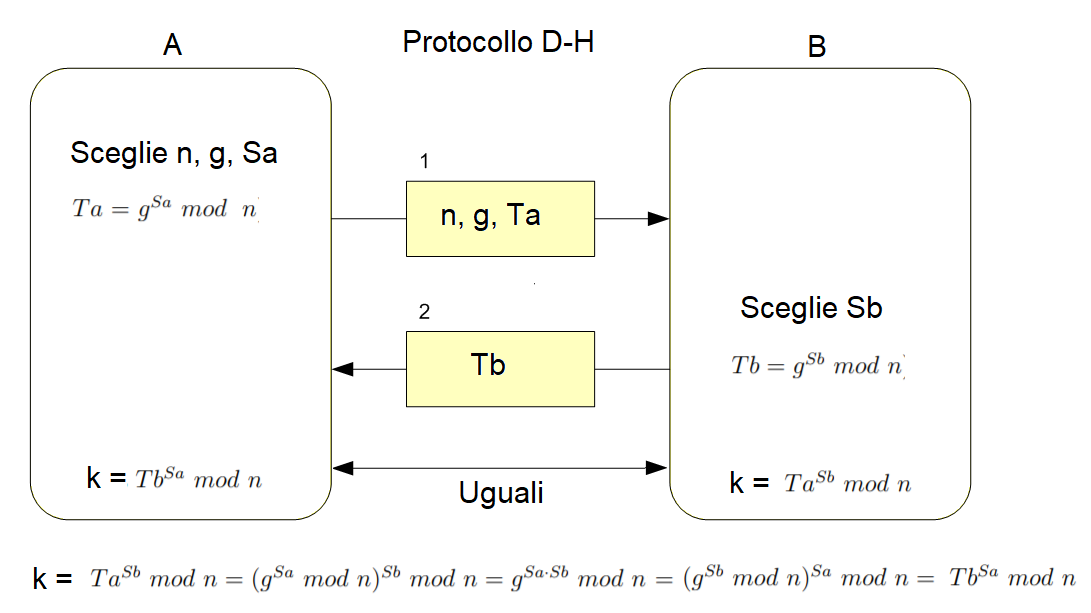
\includegraphics[width=0.8\textwidth]{MainContent/img/cap3/DH.png}
    \caption{Protocollo Diffie Hellman}
    \label{fig:DH}
\end{figure}
\begin{esempio} \\
    Con numeri semplici:
    \begin{itemize}
        \item A sceglie $n$ = 47, $g$ = 7 e $Sa$ = 10 e manda a B (47, 7, 32) perché $7^{10}$mod 47 = 32;
        \item B sceglie $Sb$ = 6 e manda ad A 8 perché $7^6$mod 47 = 8;
        \item A calcola $(8^{10})$mod 47 = 34;
        \item B calcola $(32^6)$mod 47 = 34;
    \end{itemize}
    A e B usano 34 come chiave segreta condivisa $k$.\\
    Un intruso non può calcolare $Sa$ o $Sb$ anche se intercetta $Ta = g^{Sa}$ $mod$ $n$ o $Tb = g^{Sb}$ $mod$ $n$; non si conosce nessun metodo pratico per effettuare il calcolo.
\end{esempio}
A questo punto i due interlocutori sono entrambi in possesso della chiave segreta e possono cominciare ad usarla per cifrare le comunicazioni successive.
\subsection{Sicurezza del protocollo e considerazioni}
\subsubsection{Intercettazione}
Un attaccante ("eavesdropper") può ascoltare tutto lo scambio DH, rimanendo inosservato. Invece, i protocolli di QKD sono immuni alle intercettazioni da parte di terzi, poiché i due interlocutori verrebbero a conoscenza dell'accaduto e scarterebbero le informazioni appena trasmesse.

\subsubsection{Calcolo della chiave scambiata}
Per calcolare i valori $Sa$, $Sb$, $n$, $g$ utili per calcolare la chiave $ k = g^{Sa \cdot Sb}$ $mod$ $n$, avrebbe bisogno di risolvere il problema del \textbf{logaritmo discreto}, che, come accennato in precedenza, è un processo \textbf{computazionalmente oneroso e richiede parecchio tempo}, in quanto sub-esponenziale (sicuramente molto più del tempo di conversazione tra i 2 interlocutori). Questo, oggi, (utilizzando le tecnologie tradizionali) è considerato un problema \textbf{difficile}. \\
\cite{kong_review_2022}
Con l'avvento delle tecnologie quantiche, però, non ci sono prove teoriche che lo schema Diffie-Hellman possa proteggere incondizionatamente la chiave segreta da un intercettatore con risorse quantistiche illimitate. Infatti è stato dimostrato che un computer quantistico risolve il problema del logaritmo discreto in un lasso di tempo sostanzialmente inferiore a quello impiegato da un calcolatore comune. Di conseguenza, essere in grado di calcolare in modo efficiente logaritmi discreti implica essere in grado di rompere Diffie-Hellman, il quale risulta totalmente insicuro contro un avversario che possiede tecnologie quantistiche arbitrarie. Sebbene la crittografia post-quantica possa essere utilizzata per rafforzare lo schema Diffie-Hellman, in questa relazione mi vorrei soffermare sulle tecnologie di Quantum Key Distribution, che proteggono la chiave segreta attraverso i fondamenti della fisica. Le tecnologie quantistiche trattate risolvono questo problema a monte, ovvero un attaccante viene rilevato dalle controparti non appena tenta di intercettare le informazioni scambiate attraverso il canale quantistico. L'unico attacco possibile è quello a forza bruta ma, siccome ogni chiave viene utilizzata una volta soltanto (one-time-pad), questo è poco efficace. Inoltre, i protocolli QKD non dipendono dalla complessità computazionale e, quindi, non sono a rischio di diventare obsoleti di fronte al rapido sviluppo della potenza di calcolo. \\

\subsubsection{Man in the middle}
L'algoritmo Diffie-Hellman è vulnerabile all'attacco "Man in the middle", durante il quale un agente terzo può falsificare le chiavi pubbliche di Alice e Bob ed ingannare le due parti. L'algoritmo DH infatti attua lo scambio delle chiavi simmetriche segrete, ma con il presupposto di avere delle informazioni pubbliche condivise e si dimostra resistente nei confronti dell'intercettamento di queste ultime (a partire dalle informazioni pubbliche non si riesce a ricostruire la chiave, è computazionalmente difficile). Ma nulla può impedire che le informazioni pubbliche siano state modificate o falsificate; in questo caso Alice e Bob non avrebbero modo di accorgersi della frode appoggiandosi al solo algoritmo Diffie-Hellman. Ecco perché occorre che le informazioni pubbliche, ovvero gli elementi $n, g$, possano essere autenticate tramite un algoritmo di autenticazione o da un'autorità di certificazione (CA).
In questo caso, anche i protocolli di QKD sono vulnerabili a questo tipo di attacco ed è necessario che le due parti si autentichino a vicenda per poi stabilire una connessione sicura.

\subsubsection{Forward Secrecy}
Il protocollo Diffie-Hellman è stato progettato per offrire FS, difatti ogni chiave effimera derivata è \textbf{indipendente}. Tanto è vero che, se un attaccante dovesse ricavarne una, sarà in grado di decifrare solamente la relativa conversazione ed esso non avrebbe alcuna informazione sulle altre chiavi. Questo è vero anche per il protocollo di QKD BB84.

\subsubsection{Comparazione Diffie-Hellman e Quantum Key Distribution}
\begin{table}[H]
\centering
    \begin{tabular}{|c|c|c|}
    \hline
     & D-H & QKD\\
    \hline
    Intercettazione & Vulnerabile & \makecell{Sicuro: Le due parti possono verificare \\la presenza di un intercettatore}\\
    \hline
    \makecell{Calcolo della\\chiave  condivisa}& \makecell{Vulnerabile\\(con tecnologie quantistiche)} & \makecell{Sicuro: l'unico attacco possibile è\\ l'attacco a forza bruta ma la chiave\\ viene cambiata continuamente}\\
    \hline
    \makecell{Man in the middle} & Vulnerabile & Vulnerabile\\
    \hline
    \makecell{Forward Secrecy} & Garantita & Garantita\\
    \hline
    \end{tabular}
    \caption{Comparazione tra DH e QKD}
    \label{tab:DH_vs_QKD}
\end{table}
\newpage
\section{Scambio di chiavi con RSA}
Un altro protocollo utilizzato per lo scambio di chiavi effimere è il protocollo asimmetrico RSA (Rivest–Shamir–Adleman) \cite{noauthor_rsa_2022}. RSA è basato sull'elevata complessità computazionale della fattorizzazione in numeri primi. Il suo funzionamento base è il seguente:
\begin{enumerate}
    \item si scelgono a caso due numeri primi, $p$ e $q$ abbastanza grandi da garantire la sicurezza dell'algoritmo (ad esempio, il più grande numero RSA, RSA-2048, utilizza due numeri primi lunghi più di 300 cifre).
    \item si calcola il loro prodotto $n = pq$, chiamato modulo (dato che tutta l'aritmetica seguente è modulo $n$), e il prodotto $\varphi(n)=(p-1)(q-1)$, dove
    $\varphi(n)$ è la funzione toziente.
    \item si considera che la fattorizzazione di $n$ è segreta e solo chi sceglie i due numeri primi, $p$ e $q$, la conosce.
    \item si sceglie poi un numero $e$ (chiamato esponente pubblico), coprimo con $\varphi(n)$ e più piccolo di $\varphi(n)$.
    \item si calcola il numero $d$ (chiamato esponente privato) tale che il suo prodotto con $e$ sia congruo a $1$ $mod$ $\varphi(n)$ ovvero che $ed$ $\equiv$ $1$ $mod$ $(\varphi (n))$
\end{enumerate}
La chiave pubblica è $K_{pub} = (n,e)$, mentre la chiave privata è $K_{priv}(n,d)$.
La forza dell'algoritmo sta nel fatto che per calcolare $d$ da $e$ (o viceversa) non basta la conoscenza di $n$ ma serve il numero $\varphi(n)=(p-1)(q-1)$, e che il suo calcolo richiede tempi molto elevati; infatti fattorizzare in numeri primi (cioè scomporre un numero nei suoi divisori primi) è un'operazione computazionalmente molto costosa.\\
Se Alice e Bob sono in possesso delle chiavi pubbliche dell'altro e, se volessero scambiarsi una chiave effimera segreta, il procedimento è il seguente:
\begin{enumerate}
    \item Alice genera una chiave $k$ (con generatori casuali o scelta da lei) da utilizzare in seguito come chiave simmetrica.
    \item Alice la cifra utilizzando la chiave pubblica di Bob $K_{pubB}= (e,n)$, quindi calcola il valore $c = k^e$ $mod$ $n$ e lo invia a Bob.
    \item Bob utilizza la propria chiave privata $K_{privB}= (d,n)$ per decifrare il messaggio ricevuto da Alice, quindi calcola $c^d$ $mod$ $n$ $=$ $k^{ed}$ $mod$ $n$ $=$ $k^1\;mod\;n$ $=$ $k$
\end{enumerate}
A questo punto i due interlocutori sono entrambi in possesso della chiave segreta $k$ e possono cominciare ad usarla per cifrare le comunicazioni successive.

\subsection{Sicurezza del protocollo e considerazioni}
\subsubsection{Intercettazione}
Un attaccante ("eavesdropper") può ascoltare lo scambio, ma per calcolare la chiave condivisa $k$ deve decifrare il messaggio criptato, ovvero trovare i fattori primi di $n$. Come annunciato in precedenza, questo è un calcolo incredibilmente complesso per i calcolatori comuni. Tuttavia, è stato dimostrato che l'algoritmo di \textbf{Shor} \cite{shor_polynomial-time_1997} permette di scomporre il numero $n$ nei suoi fattori primi $p$ e $q$ in tempo \textbf{polinomiale} (cioè sub-esponenziale). In questo modo, se l'attaccante avesse a disposizione risorse quantistiche arbitrarie, sarebbe in grado di "rompere" l'algoritmo RSA e di ricavare la chiave segreta scambiata tra i due interlocutori.
\subsubsection{Man in the middle}
Anche in questo caso, l'unico attacco attivo che si può pensare è il man-in-the-middle, cioè c'è la possibilità che l'attaccante si inserisca nelle comunicazioni tra Alice e Bob nel momento dello scambio delle chiavi pubbliche: questo accade perché le chiavi, di per sé, non sono autenticate. In TLS vengono utilizzati i certificati digitali a questo scopo.
\subsubsection{Osservazioni temporali o timing attack}
Si tratta di un attacco insolito ed nessuno se lo sarebbe mai aspettato quando fu standardizzato il protocollo. Si tratta, di fatto, di analizzare quanto tempo ci mette un algoritmo a decifrare una messaggio \cite{timing_attack}. Esiste, infatti, una stretta correlazione tra la chiave privata e la difficoltà computazionale richiesta per cifratura e decifratura: basta osservare quanto tempo serve ad un algoritmo per decifrare un messaggio (con la chiave pubblica) per avere alcune informazioni sulla chiave privata. Per ovviare a questo problema, le implementazioni commerciali di RSA, ad oggi, inseriscono delle attese casuali nel software, in modo da annullare la correlazione tra la firma ed il tempo necessario per decifrare i messaggi. I protocolli di QKD non sono soggetti a questo problema.
\subsubsection{Forward Secrecy}
Quando in TLS viene utilizzato RSA (e non Diffie-Hellman) per lo scambio di chiavi, per un attaccante è sufficiente ottenere la chiave privata del server per decriptare tutte le sessioni (passate e future) avviate con quel server e di conseguenza è possibile ricavare tutte le chiavi effimere scambiate tra le due parti. In sostanza, ricavando una chiave effimera l'attaccante sarà in grado di ottenere \textbf{tutte} le altre, in quanto non sono "indipendenti" (a differenza di DH). Infatti è noto come lo scambio di chiavi basato su RSA \textbf{non offra} la \textbf{forward secrecy}, ovvero la proprietà che assicura che se una chiave di cifratura a lungo termine viene compromessa, le chiavi di sessione generate a partire da essa rimangono riservate.
Questa tecnica viene attuata, ad esempio, utilizzando il popolare sniffer di rete Wireshark per ispezionare le connessioni protette da TLS.
Questo problema può essere risolto sostituendo il meccanismo RSA con il protocollo di QKD affiancato da OTP. In questo modo, nel caso in cui un eventuale attaccante dovesse in ottenere una delle chiavi effimere, sarà in grado di decifrare solamente una porzione ridotta dei messaggi scambiati, poiché le chiavi vengono cambiate di continuo (One Time Pad).

\subsubsection{Comparazione RSA e Quantum Key Distribution}
\begin{table}[H]
\centering
    \begin{tabular}{|c|c|c|}
    \hline
     & RSA & QKD\\
    \hline
    Intercettazione & Vulnerabile & \makecell{Sicuro: Le due parti possono verificare \\la presenza di un intercettatore}\\
    \hline
    \makecell{Calcolo della\\chiave  condivisa}& \makecell{Vulnerabile\\(con tecnologie quantistiche)} & \makecell{Sicuro: l'unico attacco possibile è\\ l'attacco a forza bruta ma la chiave\\ viene cambiata continuamente}\\
    \hline
    \makecell{Man in the middle} & Vulnerabile & Vulnerabile\\
    \hline
    \makecell{Timing attack} & Vulnerabile & Sicuro\\
    \hline
    \makecell{Forward Secrecy} & Non garantita & Garantita\\
    \hline
    \end{tabular}
    \caption{Comparazione tra RSA e QKD}
    \label{tab:RSA_vs_QKD}
\end{table}